% !TEX program = xelatex
\documentclass{beamer}

\usepackage{amsmath, amssymb}
% \usepackage[utf8]{inputenc}
\usepackage{zxjatype}
\usepackage[ipa]{zxjafont}
\usepackage{mymacro}
% \usepackage{qrcode}
\usepackage{listings}
\usepackage{graphicx}
\graphicspath{ {./Pictures/} }

\usefonttheme{professionalfonts}  
\setbeamertemplate{navigation symbols}{}  

% \usetheme{Frankfurt}
% \usecolortheme{seagull} % beaver
% \usebackgroundtemplate{
% \includegraphics[width=\paperwidth,
% height=\paperheight]{Page_169}
% }

% --- page number ---
\setbeamertemplate{footline}{%
	\raisebox{10pt}{\makebox[\paperwidth]{\hfill\makebox[7em]{\normalsize\texttt{\insertframenumber/\inserttotalframenumber}}}}%
}

% Presenter's note
% \setbeameroption{show notes on second screen}

\title{Python 101}
\author{Michael}
\date{\today}

\begin{document}

    \begin{frame}[plain]
        \maketitle
    \end{frame}

    \begin{frame}
        \color{blue} \Large Outline  \\
        \color{black} \normalsize \vskip 10pt 
        \begin{itemize}
            \item What is python
            \item Variable and \texttt{print()}
            \item Arithmetic and Bitwise Operator
            \item Statement and Condition
            \item Function
            \item List
            \item For Loop and While Loop
            \item Dictionary
            \item Conclusion
        \end{itemize}
    \end{frame}

    \begin{frame}
        \begin{center}
            {\color{blue} \LARGE How to use Jupyter Lab ?}
        \end{center}
    \end{frame}

    \begin{frame}[plain]
        \begin{center}
            {\color{blue} \LARGE 1 What is Python}
        \end{center}
    \end{frame}

    \begin{frame}
        Python is a high-level general-purpose programming language created by Guido
        van Rossum in 1989. It is one of the most popular programming languages in the world
    \end{frame}

    \begin{frame}
        \begin{center}
            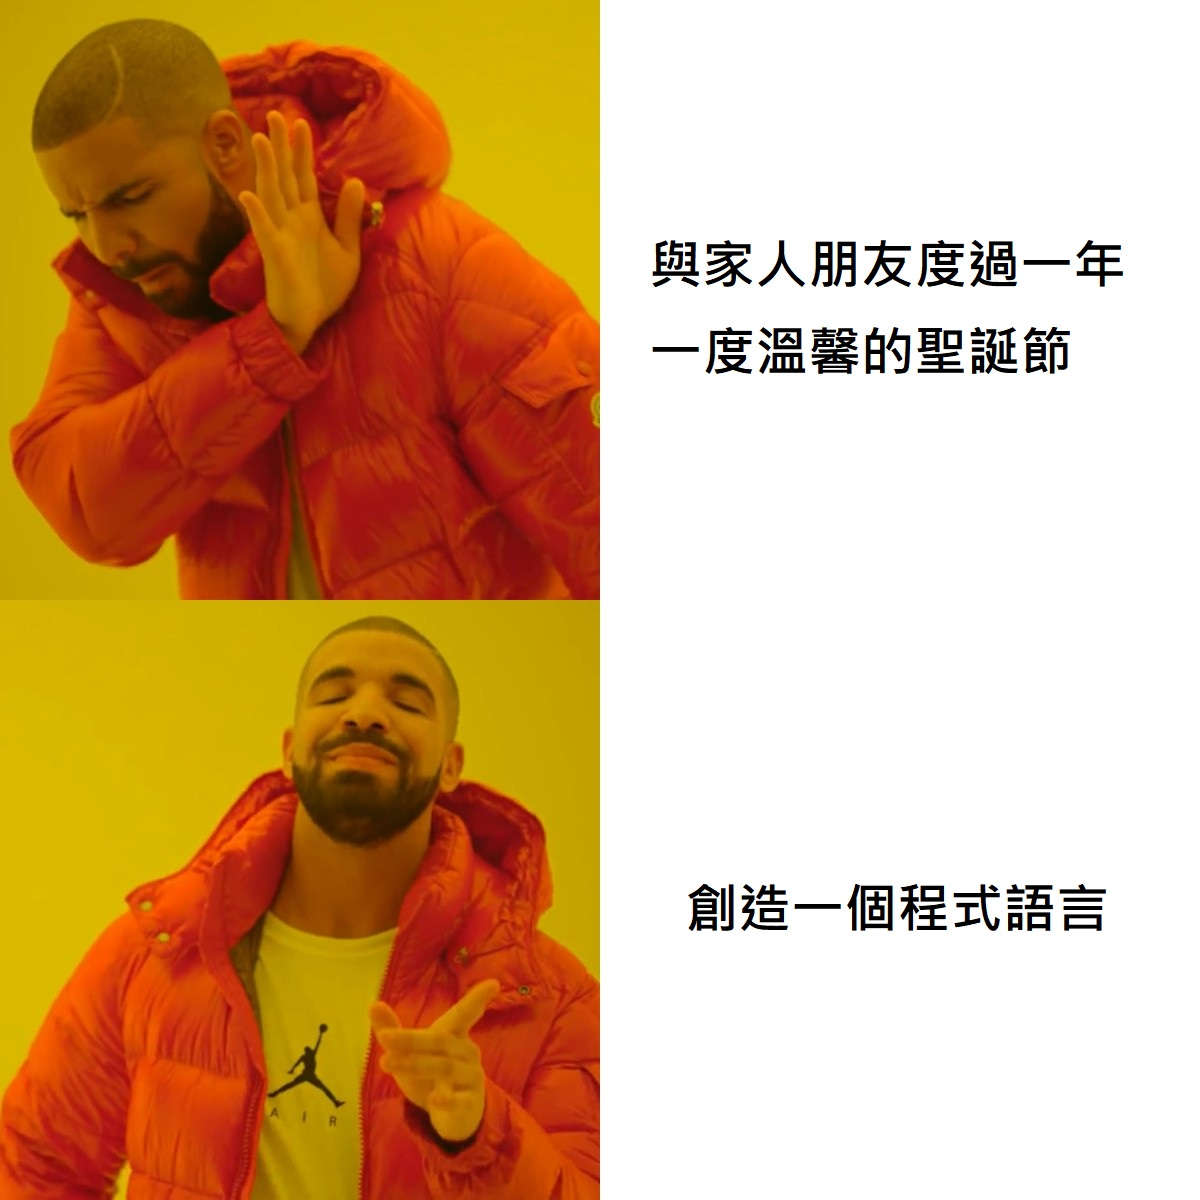
\includegraphics[scale=0.25]{Drake-Hotline-Bling.jpg}
        \end{center}
    \end{frame}

    \begin{frame}
        \color{blue} \Large 1.1 Why Python ?  \\
        
        \color{black} \normalsize \vskip 10pt 
        \begin{itemize}
            \item Works on different OS 
            \item Simple syntax
            \item Runs on interpreter systems
            \item Hundreds of libraries
            \item Can be applied to various fields
        \end{itemize}
    \end{frame}

    \begin{frame}
        \color{blue} \Large 1.2 What can Python do ?  \\
        
        \color{black} \normalsize \vskip 10pt 
        \begin{itemize}
            \item Statistical analysis
            \item Backend (server) of web applications
            \item AI and machine learning
            \item Software applications
        \end{itemize}
    \end{frame}
    
    \begin{frame}[plain,c]
        \begin{center}
            {\color{blue} \LARGE 2 Variables and \texttt{print()}}
        \end{center}
        
    \end{frame}
    
    \begin{frame}{Variables and \texttt{print()}}
        %\newline
        \color{blue} \Large 2.1 Variables \\
        
        \color{black} \normalsize \vskip 10pt As a coder, we need ``variables'' to store some data for further use. 
        Here are some basic data types :
        \begin{itemize}
            \item Integers (We will focus on this !)
            \item Floating-Point Numbers
            \item Complex Numbers
            \item Strings
            \item Boolean Type
        \end{itemize}
        
        \note{
        There are many data types, one of which is integer, abbreviated \texttt{int}, in Python. We will focus on this data type today. Nevertheless, we still list some basic data types here for your further studying
        }
    \end{frame}
    
    \begin{frame}{Variables and \texttt{print()}}
        \color{blue} \Large 2.2 \texttt{print()} \\
        \color{black} \normalsize \vskip 10pt \texttt{print()} is a function helping us to display the value of a variable.
        
    \end{frame}
    
    \begin{frame}[fragile]{Variables and \texttt{print()}}
        \color{blue} \Large 2.2.1 Example \\
        \color{black} \normalsize \vskip 10pt
        \begin{verbatim}
            a = int(3)
            b = int(5)
            print(b)
            print(a)
        \end{verbatim}

    \end{frame}
        
    \begin{frame}{Variables and \texttt{print()}}
        \color{blue} \Large 2.3 Formatted \texttt{print} \\
        \color{black} \normalsize \vskip 10pt
        We can print a formatted string (A string inside \texttt{f''} or \texttt{f""})\\
        You can refer to Python variables between \{ and \}
    \end{frame}

    \begin{frame}[fragile]{Variables and \texttt{print()}}
        \begin{verbatim}
            a = int(3)
            b = str('Michael')
            print(f'The value of a is {a}')
            print(f'my name is {b}')
        \end{verbatim}
    \end{frame} 

    % \begin{frame}{Variables and \texttt{print()}}
    %     Now, we believe you come familiar with the assignment operator \texttt{=} and a function \texttt{print()}. Wait... what do I mean by ``operator''?
    % \end{frame}
    
    \begin{frame}[plain,c]
        \begin{center}
            {\color{blue} \LARGE 3. Arithmetic and Bitwise Operators}
        \end{center}
        
    \end{frame}
    
    \begin{frame}{Arithmetic and Bitwise Operators}
        \color{blue} \Large 3.1 Arithmetic Operators \\
        
        \color{black} \normalsize \vskip 10pt 
        \begin{itemize}
            \item \texttt{+}
            \item \texttt{-}
            \item \texttt{*}
            \item \texttt{//}
            \item \texttt{**}
        \end{itemize}
    \end{frame}

    \begin{frame}[fragile]{Arithmetic and Bitwise Operators}
        \color{blue} \Large Example \\
        \color{black} \normalsize \vskip 10pt 
        \begin{verbatim}
            a = 987
            print(a)
            a = a - 87
            print(a)
            print(a // 5)
            print(3 ** 3)
        \end{verbatim}
        
    \end{frame}
    
    \begin{frame}{Arithmetic and Bitwise Operators}
        \color{blue} \Large 3.2 Bitwise Operators \\
        
        \color{black} \normalsize \vskip 10pt 
        Before going into this subsection, we need to understand what binary 
        representation is.
    
    \end{frame}
    
    \begin{frame}{Arithmetic and Bitwise Operators}
        \color{blue} \Large Binary Representation
        \color{black} \normalsize \vskip 10pt
        In decimal representation, 7050 is actually
        \[ 7 \times 10^3 + 0 \times 10^2 + 5 \times 10^1 + 0 \times 10^0 \]
        \vskip 30pt
        What if the base is not 10 ?
    \end{frame}
    
    \begin{frame}{Arithmetic and Bitwise Operators}
        \color{blue} \Large Exercise 1 \\
        \color{black} \normalsize \vskip 10pt
        What is the binary representation of 32 ?
        \note{100000}
    \end{frame}

    \begin{frame}{Arithmetic and Bitwise Operators}
        $$ 0 \times 2^0 + 0 \times 2^1 + 0 \times 2^2 + 0 \times 2^3
        + 0 \times 2^4 + 1 \times 2^5 = 32 $$
        $$ 100000 $$
    \end{frame}
    
    \begin{frame}{Arithmetic and Bitwise Operators}
        \color{blue} \Large Exercise 2 \\
        \color{black} \normalsize \vskip 10pt
        What is the binary representation of 102 ?
        \note{1100110}
    \end{frame}

    \begin{frame}{Arithmetic and Bitwise Operators}
        $$ 0 \times 2^0 + 1 \times 2^1 + 1 \times 2^2 + 0 \times 2^3
        + 0 \times 2^4 + 1 \times 2^5 + 1 \times 2^6 = 102 $$
        $$ 1100110 $$
    \end{frame}
    
    \begin{frame}{Arithmetic and Bitwise Operators}
        \color{blue} \Large List of Bitwise Operators \\
        \color{black} \normalsize \vskip 10pt
        
        \begin{itemize}
            \item \texttt{\&}
            \item \texttt{|}
            \item \texttt{\^}
            \item \texttt{>>}
            \item \texttt{<<}
        \end{itemize}
    \end{frame}

    \begin{frame}{Arithmetic and Bitwise Operators}
        \color{blue} \Large Bitwise AND \\
        \color{black} \normalsize \vskip 10pt
        The bitwise operator AND($\&$) would output the intersection of the two numbers.\\
    \end{frame}
    
    \begin{frame}{Arithmetic and Bitwise Operators}
        \begin{center}
            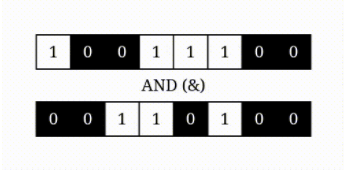
\includegraphics[scale = 0.8]{AND Before.png}
        \end{center}
        \note{156 and 52}
    \end{frame}
    
    \begin{frame}{Arithmetic and Bitwise Operators}
        \begin{center}
            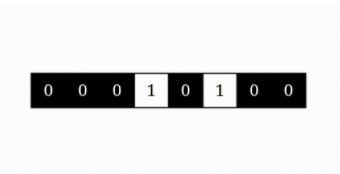
\includegraphics[scale = 0.8]{AND After.png}
        \end{center}
        \note{20}
    \end{frame}
    
    \begin{frame}{Arithmetic and Bitwise Operators}
        \color{blue} \Large Bitwise  OR\\
        \color{black} \normalsize \vskip 10pt
        
    \end{frame}
    
    \begin{frame}{Arithmetic and Bitwise Operators}
        \begin{center}
            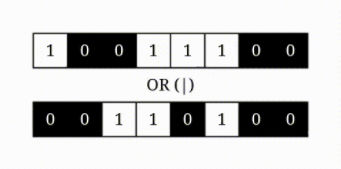
\includegraphics[scale = 0.8]{OR Before.png}
        \end{center}
        \note{156 and 52}
    \end{frame}
    
    \begin{frame}{Arithmetic and Bitwise Operators}
        \begin{center}
            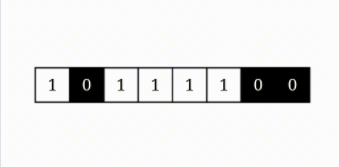
\includegraphics[scale = 0.8]{OR After.png}
        \end{center}
        \note{188}
    \end{frame}
    

    \begin{frame}{Arithmetic and Bitwise Operators}
        \color{blue} \Large Bitwise  XOR\\
        \color{black} \normalsize \vskip 10pt
    \end{frame}
    
    \begin{frame}{Arithmetic and Bitwise Operators}
        \begin{center}
            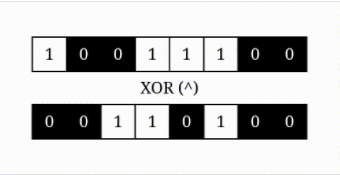
\includegraphics[scale = 0.8]{XOR Before.png}
        \end{center}
        \note{156 and 52}
    \end{frame}
    
    \begin{frame}{Arithmetic and Bitwise Operators}
        \begin{center}
            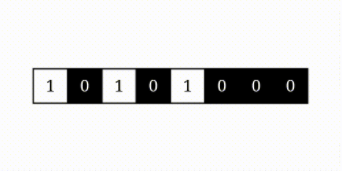
\includegraphics[scale = 0.8]{XOR After.png}
        \end{center}
        \note{168}
    \end{frame}

    \begin{frame}{Arithmetic and Bitwise Operators}
        \begin{center}
            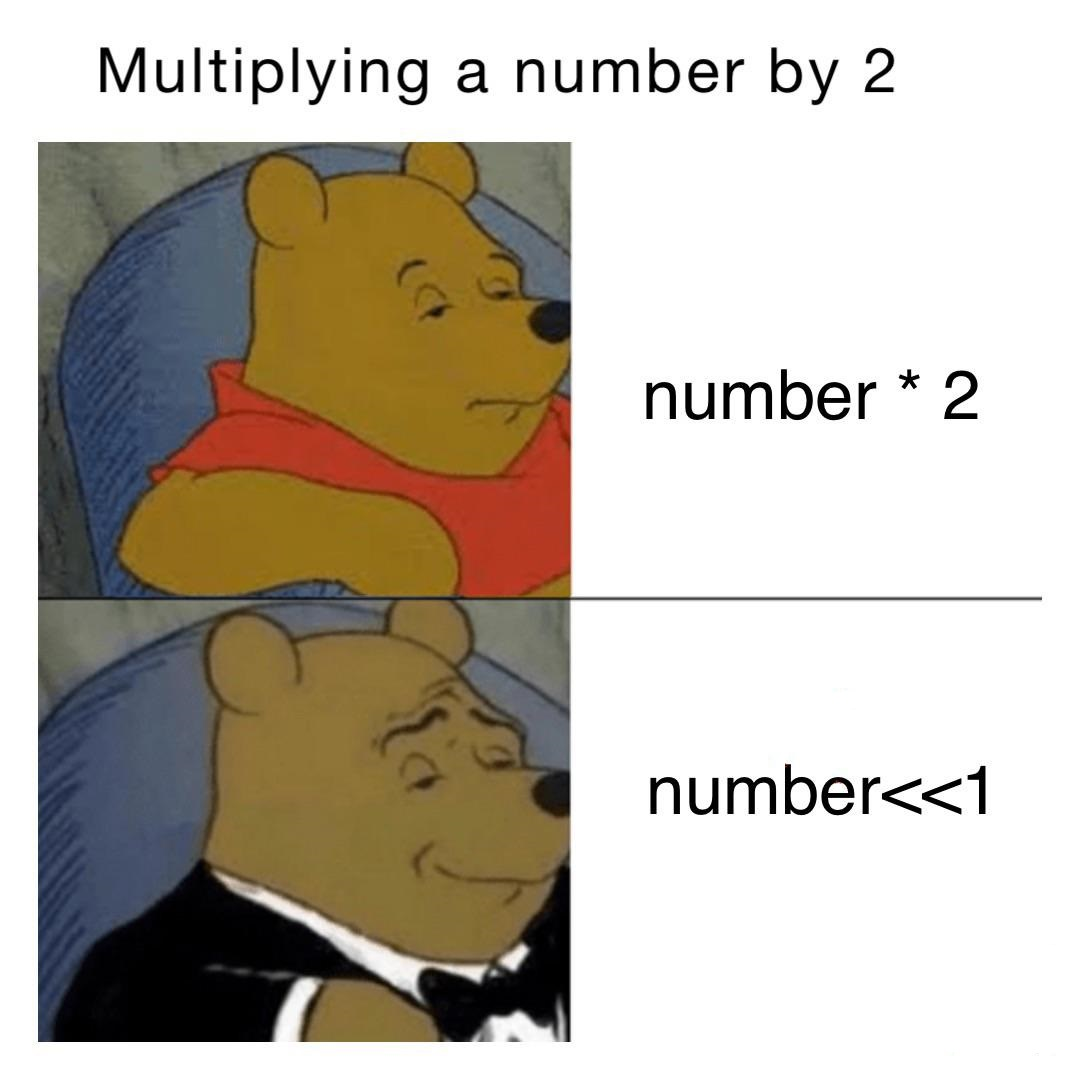
\includegraphics[scale = 0.25]{Bitwise_meme.jpg}
        \end{center}
    \end{frame}

    \begin{frame}{Arithmetic and Bitwise Operators}
        \color{blue} \Large Assignment Operators \\
        \color{black} \normalsize \vskip 10pt
        \begin{itemize}
            \item \texttt{=}
            \item \texttt{+=}
            \item $\vdots$
            \item \texttt{//=}
            \item \texttt{\&=}
            \item $\vdots$
            \item \texttt{<<=}
        \end{itemize}
    \end{frame}

    \begin{frame}[fragile]{Arithmetic and Bitwise Operators}
        \color{blue} \Large Example \\
        \color{black} \normalsize \vskip 10pt
        \begin{verbatim}
            a = 5
            a = a + 5
            print(a)
            a += 5
            print(a)
        \end{verbatim}
    \end{frame}

    \begin{frame}[plain, c]
        \begin{center}
            \color{blue} \LARGE 4 Statement and Conditions
        \end{center}
    \end{frame}
    
    \begin{frame}{Statement and Conditions}
        Sometimes, we may want our program do different things based on different conditions. \\
        \begin{itemize}
            \item \texttt{if}
            \item \texttt{else}
            \item \texttt{elif}
        \end{itemize}
    \end{frame}

    \begin{frame}[fragile]{Statement and Conditions}
        \color{blue} \Large Example \\
        \color{black} \normalsize \vskip 10pt
        \begin{verbatim}
            a = 529
            if (a % 2 == 0):
                print("Even")
            else :
                print("Odd")
        \end{verbatim}
    \end{frame}

    \begin{frame}{Statement and Conditions}
        Moreover, things are usually complicated so we need some ``conjunctions''.
        \begin{itemize}
            \item \texttt{and}
            \item \texttt{or}
        \end{itemize}
    \end{frame}

    \begin{frame}[fragile]{Statement and Conditions}
        \color{blue} \Large Example \\
        \color{black} \normalsize \vskip 10pt
        \begin{verbatim}
    a = 200
    b = 33
    c = 500
    if (a > b and c > a) :
        print("Both conditions are True")
    if (b < a or c < a) :
        print("At least one of the conditions is True")
        \end{verbatim}  
    \end{frame}

    
    \begin{frame}{Statement and Conditions}
        \color{blue} \Large Exercise \\
        \color{black} \normalsize \vskip 5pt
        Write a program to check whether a number is between 1500 and 2700, then check 
        if it's divisible by 7 or 5. If not, your program need to output whether the 
        number is "Out of range" or "Not divisible".
    \end{frame}
    
    \begin{frame}{Statement and Conditions}
        \color{blue} \Large Hints \\
        \color{black} \normalsize \vskip 5pt
        \begin{enumerate}
            \item Store the number in a variable
            \item Write a if statement to check whether the number is in range
            \item Write a if statement inside the previous one and check if the number is divisible by 7 or 5
            \item print anything you want if both statement is true
            \item Figure out the rest by yourself !
        \end{enumerate}
    \end{frame}

    \begin{frame} [fragile] {Statement and Conditions}
        \color{blue} \Large Answer \\
        \color{black} \normalsize \vskip 10pt
        \begin{verbatim}
            a = 438
            if (a >= 1500 and a <= 2700) :
                if (a % 7 == 0 or a % 5 == 0):
                    print("Test successful")
                else :
                    print("Not divisible")
            else:
                print("Out of range!")
        \end{verbatim}
    \end{frame}

    \begin{frame}[plain, c]
        \begin{center}
            \color{blue} \LARGE 5 Functions
        \end{center}
    \end{frame}
    
    \begin{frame}{Functions}
        \color{blue} \Large What are Functions \\
        \color{black} \normalsize \vskip 5pt
        A function is a block of code that does certain calculations and return the result to you.\\
    \end{frame}
    
    \begin{frame}{Functions}
        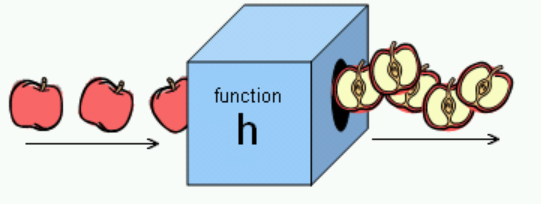
\includegraphics[scale = 0.7]{Functions.png}
    \end{frame}
    
    \begin{frame}[fragile]{Functions}
        \color{blue} \Large Example \\
        \color{black} \normalsize \vskip 5pt
        \begin{verbatim}
            def myFunction(num1, num2) :
                return num1**2 + num2**2
        \end{verbatim}
    \end{frame}
    
    \begin{frame}{Functions}
        \color{blue} \Large Why Functions? \\
        \color{black} \normalsize \vskip 5pt
        \begin{itemize}
            \item Don't have to copy and paste your code everywhere
            \item Prevent inconsistency
            \item Easy to manage
        \end{itemize}
    \end{frame}

    \begin{frame}[fragile]{Functions}
        \color{blue} \Large If we dont use functions... \\
        \color{black} \normalsize \vskip 5pt
        \begin{verbatim}
            print("Cherry, Happy New year !")
            print("Brian, Happy New Year !")
            print("Hubert, Happy New Year !")
            print("Tommy, Happy New Year !")
        \end{verbatim}
    \end{frame}

    \begin{frame}[fragile]{Functions}
        \color{blue} \Large With functions\\
        \color{black} \normalsize \vskip 5pt
        \begin{verbatim}
            def greetings(name):
                print(f"{name}, Happy New Year !")
            greetings("Cherry")
            greetings("Brian")
            greetings("Hubert")
            greetings("Tommy")
        \end{verbatim}
    \end{frame}

    \begin{frame}
        \begin{center}
            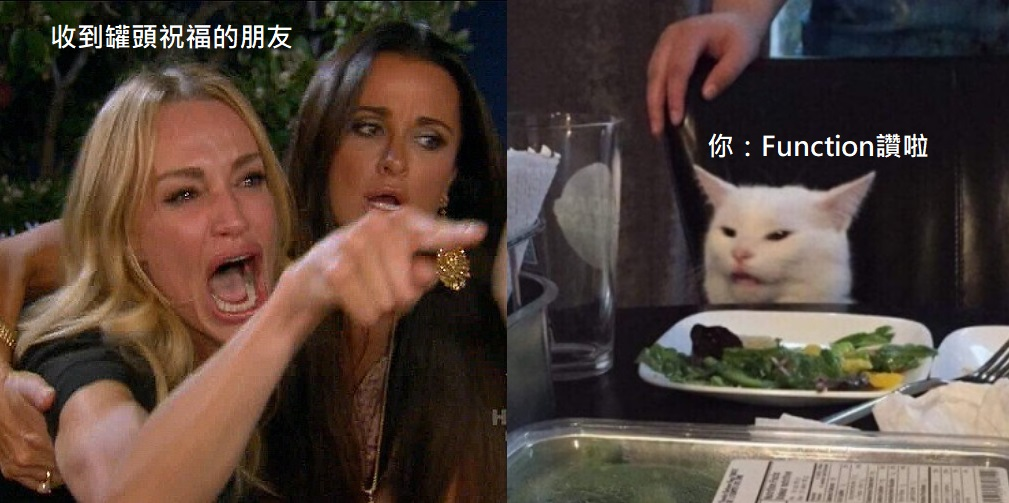
\includegraphics[scale=0.3]{Cat_and_women.jpg}
        \end{center}
    \end{frame}
    
    \begin{frame}{Functions}
        \color{blue} \Large Exercise \\
        \color{black} \normalsize \vskip 5pt
        We define $A \oplus B = A \times B + A$, \\
        write a Python code to calculate $ (10 \oplus 4) * (5 \oplus 8) - (2^8) $ \\
        (Requirement : Define a function \texttt{oplus} to do $\oplus$ operation)
    \end{frame}
    
    \begin{frame}[fragile]{Functions}
        \color{blue} \Large Answer \\
        \color{black} \normalsize \vskip 5pt
        \begin{verbatim}
        def oplus (A, B):
            return (A * B + A)
        print (oplus(10, 4) * oplus(5, 8) - 2**8)
        # 1994
        \end{verbatim}
    \end{frame} 
    
    \begin{frame}[plain, c]
    \begin{center}
        \color{blue} \LARGE 6 Lists
    \end{center}
    \end{frame}

    \begin{frame}[fragile]{Lists}
        \color{blue} \Large Motivation \\
        \color{black} \normalsize \vskip 5pt
        Suppose that we have 5 numbers \\
        How do we store it ? \\
        \begin{verbatim}
            num1 = 3
            num2 = 6
            num3 = 23
            num4 = 97
            num5 = 7414
        \end{verbatim}
    \end{frame}

    \begin{frame}{Lists}
        What if there are 1000 numbers ?
        \vskip 20pt 
        We can put them inside a \texttt{list} !
    \end{frame}
    
    \begin{frame}{Lists}
        \color{blue} \Large Constructing a List \\
        \color{black} \normalsize \vskip 5pt
        Lists can be created using square brackets.\\
        \texttt{my\_list = [5, 60, 95, 33, 83]} \\ 
        Or you could use \texttt{list()} : 
        \begin{itemize}
            \item \texttt{list()} $\Rightarrow$ []
            \item \texttt{list([1, 2, 3])} $\Rightarrow$ [1, 2, 3]
            \item \texttt{list(range(5))} $\Rightarrow$ [0, 1, 2, 3, 4]
            \item \texttt{list(range(0, 10, 2))} $\Rightarrow$ [0, 2, 4, 6, 8]
        \end{itemize}
    \end{frame}

    \begin{frame}{List}
        \begin{center}
            
\includegraphics[scale=0.6]{Who_are_you.png}
        \end{center}
        
    \end{frame}

    \begin{frame}{List}
        \color{blue} \Large Range Functions ! \\
        \color{black} \normalsize \vskip 10pt
        It creates a sequence of numbers
        \begin{itemize}
            \item \texttt{range(6)} $\rightarrow$ \texttt{[0, 1, 2, 3, 4, 5]}
            \item \texttt{range(1, 7, 2)} $\rightarrow$ \texttt{[1, 3, 5]} (No 7 !)
        \end{itemize}
    \end{frame}
    
    \begin{frame}{Lists}
        We use "index" to access elements in a list. \\
        The first item in lists has index 0, the second item has index 1, etc.\\
        For example, we can use \texttt{my\_list[2]} to access the third element\\
        in the list.
    \end{frame}
    
    \begin{frame}{Lists}
        \color{blue} \Large Examples \\
        \color{black} \normalsize
        L = [5, 10, 15, 20, 25, 30, 35, 40, 45, 50] \\
        \begin{align*}
            \texttt{L[2]} & \Rightarrow 15 \\
            \texttt{L[-2]} & \Rightarrow 45 \\
            \texttt{L[2:5]} & \Rightarrow [15, 20, 25] \\
            \texttt{L[:3]} & \Rightarrow [5, 10, 15] \\
            \texttt{L[6:]} & \Rightarrow [35, 40, 45, 50] \\
        \end{align*}
    \end{frame}
    
    \begin{frame}{Lists}
        \color{blue} \Large Add or Remove Elements \\
        \color{black} \normalsize \vskip 5pt
        \begin{itemize}
            \item Use \texttt{append()} to add element to the end of the list. \\
                  e.g. \texttt{my\_list.append(50)} 
            \item Use \texttt{insert()} to add element to a specific index of the list. \\
                  e.g. \texttt{my\_list.insert(i, elem)}
            \item Use \texttt{remove()} to remove an element in the list. \\
                  e.g. \texttt{my\_list.remove(60)}
            \item Use \texttt{pop()} to remove an element in a specific index. \\
                  e.g. \texttt{my\_list.pop(1)}
        \end{itemize}
        
    \end{frame}
    
    \begin{frame}{Lists}
        \color{blue} \Large Some Functions of Lists \\
        \color{black} \normalsize \vskip 5pt
        \begin{align*}
            \texttt{len([5, 3, 1])} &\Rightarrow 3 \\
            \texttt{max([1, 2, 3, 4, 5])} &\Rightarrow 5 \\
            \texttt{min([0, 55, 3, 75])} &\Rightarrow 0 \\
            \texttt{sum([1, 2, 3, 4, 5])} &\Rightarrow 15 \\
        \end{align*}
    \end{frame}

    \begin{frame}{Lists}
        \color{blue} \Large Exercise \\
        \color{black} \normalsize \vskip 10pt
        Write a python program to find and remove the largest number in 
        a list, and insert the sum of the list at the end.
    \end{frame}

    \begin{frame}[fragile]{Lists}
        \color{blue} \Large Answer \\
        \color{black} \normalsize \vskip 10pt
        \begin{verbatim}
            numbers = [15, 67, 23, 99, 25, 44, 73]
            maximum = max(numbers)
            numbers.remove(maximum)
            numbers.append(sum(numbers))
            print(numbers)
        \end{verbatim}
    \end{frame}
    
    \begin{frame}[plain, c]
        \begin{center}
            \color{blue} \LARGE 7 For Loop and While Loop
        \end{center}
    \end{frame}
    
    \begin{frame}[fragile]{For Loop and While Loop}
        \color{blue} \Large For Loop \\
        \color{black} \normalsize \vskip 5pt
        We can use for loops to make our program do repetitive things \\
        e.g. add from 1 to 5 \\
        \begin{verbatim}
            num = 0
            for i in range (1, 6):
               num += i
            print (num)
        \end{verbatim}
    \end{frame}
    
    \begin{frame}[fragile]{For Loop and While Loop}
        You could also use it to iterate through a list
        \begin{verbatim}
            L = [5, 2, 88]
            for i in L :
               print (i)
        \end{verbatim}
    \end{frame}
    
    \begin{frame}[fragile]{For Loop and While Loop}
        \color{blue} \Large While Loop \\
        \color{black} \normalsize \vskip 5pt
        Execute a set of statements as long as a condition is true.\\
        \begin{verbatim}
            i = 0
            while (i < 5):
               print (i)
               i += 1
        \end{verbatim}
    \end{frame}
    
    \begin{frame}{For Loop and While Loop}
        \color{blue} \Large Break \\
        \color{black} \normalsize \vskip 5pt
        We use \texttt{break()} to break out of a loop. \\
    \end{frame}
    
    \begin{frame}{For Loop and While Loop}
        \color{blue} \Large Continue \\
        \color{black} \normalsize \vskip 5pt
        We use \texttt{continue} to skip rest of the code and start a new iteration. \\
    \end{frame}
    
    \begin{frame}{For Loop and While Loop}
        \color{blue} \Large Exercise \\
        \color{black} \normalsize \vskip 5pt
        Write a python code to print from $1 \times 1$ to $9 \times 9$
    \end{frame}
    
    \begin{frame}[fragile]{For Loop and While Loop}
        \color{blue} \Large Answer \\
        \color{black} \normalsize \vskip 5pt
        \begin{verbatim}
        for i in range (1, 10):
            for j in range (1, 10):
                print(f'{i} x {j} = {i*j}')
            print('\n')
        \end{verbatim}
    \end{frame}

    \begin{frame}
        \begin{center}
            \color{blue} \LARGE Dictionary
        \end{center}
    \end{frame}

    \begin{frame}{Dictionary}
        Suppose we have a list that stores informations about a person. \\
        \texttt{["Michael","Chen","NTU","IM","Clown","2001-4-19"]}
    \end{frame}

    \begin{frame}{Dictionary}
        What attribute does each index represents ?
        \vskip 20pt 
        Dictionary can help you !
    \end{frame}

    \begin{frame}[fragile]{Dictionary}
        \begin{verbatim}
            thisDict = {
                "First_name": "Michael",
                "Last_name": "Chen",
                "School": "NTU",
                "Department": "IM",
                "Job": "Clown",
                "Birthday": "2001-4-19"
            }
        \end{verbatim}
    \end{frame}
    
    \begin{frame}[plain, c]
        \begin{center}
            \color{blue} \LARGE Conclusion
        \end{center}
    \end{frame}
    
    \begin{frame}{Conclusion}
        Now that you've learned the basic syntax for Python, \\
        you can explore various packages for Python ! \\
        For example, \texttt{numpy, pandas, matplotlib, scipy}... \\
        
    \end{frame}
    
    \begin{frame}[plain, c]
        \begin{center}
            \color{blue} \LARGE Thank You For Listening !
        \end{center}
    \end{frame}

\end{document}
